% Options for packages loaded elsewhere
\PassOptionsToPackage{unicode}{hyperref}
\PassOptionsToPackage{hyphens}{url}
\PassOptionsToPackage{dvipsnames,svgnames,x11names}{xcolor}
%
\documentclass[
]{article}

\usepackage{amsmath,amssymb}
\usepackage{iftex}
\ifPDFTeX
  \usepackage[T1]{fontenc}
  \usepackage[utf8]{inputenc}
  \usepackage{textcomp} % provide euro and other symbols
\else % if luatex or xetex
  \usepackage{unicode-math}
  \defaultfontfeatures{Scale=MatchLowercase}
  \defaultfontfeatures[\rmfamily]{Ligatures=TeX,Scale=1}
\fi
\usepackage{lmodern}
\ifPDFTeX\else  
    % xetex/luatex font selection
  \setmainfont[]{Latin Modern Roman}
  \setmathfont[]{Latin Modern Math}
\fi
% Use upquote if available, for straight quotes in verbatim environments
\IfFileExists{upquote.sty}{\usepackage{upquote}}{}
\IfFileExists{microtype.sty}{% use microtype if available
  \usepackage[]{microtype}
  \UseMicrotypeSet[protrusion]{basicmath} % disable protrusion for tt fonts
}{}
\makeatletter
\@ifundefined{KOMAClassName}{% if non-KOMA class
  \IfFileExists{parskip.sty}{%
    \usepackage{parskip}
  }{% else
    \setlength{\parindent}{0pt}
    \setlength{\parskip}{6pt plus 2pt minus 1pt}}
}{% if KOMA class
  \KOMAoptions{parskip=half}}
\makeatother
\usepackage{xcolor}
\setlength{\emergencystretch}{3em} % prevent overfull lines
\setcounter{secnumdepth}{5}
% Make \paragraph and \subparagraph free-standing
\ifx\paragraph\undefined\else
  \let\oldparagraph\paragraph
  \renewcommand{\paragraph}[1]{\oldparagraph{#1}\mbox{}}
\fi
\ifx\subparagraph\undefined\else
  \let\oldsubparagraph\subparagraph
  \renewcommand{\subparagraph}[1]{\oldsubparagraph{#1}\mbox{}}
\fi


\providecommand{\tightlist}{%
  \setlength{\itemsep}{0pt}\setlength{\parskip}{0pt}}\usepackage{longtable,booktabs,array}
\usepackage{calc} % for calculating minipage widths
% Correct order of tables after \paragraph or \subparagraph
\usepackage{etoolbox}
\makeatletter
\patchcmd\longtable{\par}{\if@noskipsec\mbox{}\fi\par}{}{}
\makeatother
% Allow footnotes in longtable head/foot
\IfFileExists{footnotehyper.sty}{\usepackage{footnotehyper}}{\usepackage{footnote}}
\makesavenoteenv{longtable}
\usepackage{graphicx}
\makeatletter
\def\maxwidth{\ifdim\Gin@nat@width>\linewidth\linewidth\else\Gin@nat@width\fi}
\def\maxheight{\ifdim\Gin@nat@height>\textheight\textheight\else\Gin@nat@height\fi}
\makeatother
% Scale images if necessary, so that they will not overflow the page
% margins by default, and it is still possible to overwrite the defaults
% using explicit options in \includegraphics[width, height, ...]{}
\setkeys{Gin}{width=\maxwidth,height=\maxheight,keepaspectratio}
% Set default figure placement to htbp
\makeatletter
\def\fps@figure{htbp}
\makeatother
% definitions for citeproc citations
\NewDocumentCommand\citeproctext{}{}
\NewDocumentCommand\citeproc{mm}{%
  \begingroup\def\citeproctext{#2}\cite{#1}\endgroup}
\makeatletter
 % allow citations to break across lines
 \let\@cite@ofmt\@firstofone
 % avoid brackets around text for \cite:
 \def\@biblabel#1{}
 \def\@cite#1#2{{#1\if@tempswa , #2\fi}}
\makeatother
\newlength{\cslhangindent}
\setlength{\cslhangindent}{1.5em}
\newlength{\csllabelwidth}
\setlength{\csllabelwidth}{3em}
\newenvironment{CSLReferences}[2] % #1 hanging-indent, #2 entry-spacing
 {\begin{list}{}{%
  \setlength{\itemindent}{0pt}
  \setlength{\leftmargin}{0pt}
  \setlength{\parsep}{0pt}
  % turn on hanging indent if param 1 is 1
  \ifodd #1
   \setlength{\leftmargin}{\cslhangindent}
   \setlength{\itemindent}{-1\cslhangindent}
  \fi
  % set entry spacing
  \setlength{\itemsep}{#2\baselineskip}}}
 {\end{list}}
\usepackage{calc}
\newcommand{\CSLBlock}[1]{\hfill\break\parbox[t]{\linewidth}{\strut\ignorespaces#1\strut}}
\newcommand{\CSLLeftMargin}[1]{\parbox[t]{\csllabelwidth}{\strut#1\strut}}
\newcommand{\CSLRightInline}[1]{\parbox[t]{\linewidth - \csllabelwidth}{\strut#1\strut}}
\newcommand{\CSLIndent}[1]{\hspace{\cslhangindent}#1}

\usepackage{arxiv}
\usepackage{orcidlink}
\usepackage{amsmath}
\usepackage[T1]{fontenc}
\makeatletter
\@ifpackageloaded{caption}{}{\usepackage{caption}}
\AtBeginDocument{%
\ifdefined\contentsname
  \renewcommand*\contentsname{Table of contents}
\else
  \newcommand\contentsname{Table of contents}
\fi
\ifdefined\listfigurename
  \renewcommand*\listfigurename{List of Figures}
\else
  \newcommand\listfigurename{List of Figures}
\fi
\ifdefined\listtablename
  \renewcommand*\listtablename{List of Tables}
\else
  \newcommand\listtablename{List of Tables}
\fi
\ifdefined\figurename
  \renewcommand*\figurename{Figure}
\else
  \newcommand\figurename{Figure}
\fi
\ifdefined\tablename
  \renewcommand*\tablename{Table}
\else
  \newcommand\tablename{Table}
\fi
}
\@ifpackageloaded{float}{}{\usepackage{float}}
\floatstyle{ruled}
\@ifundefined{c@chapter}{\newfloat{codelisting}{h}{lop}}{\newfloat{codelisting}{h}{lop}[chapter]}
\floatname{codelisting}{Listing}
\newcommand*\listoflistings{\listof{codelisting}{List of Listings}}
\makeatother
\makeatletter
\makeatother
\makeatletter
\@ifpackageloaded{caption}{}{\usepackage{caption}}
\@ifpackageloaded{subcaption}{}{\usepackage{subcaption}}
\makeatother
\ifLuaTeX
  \usepackage{selnolig}  % disable illegal ligatures
\fi
\usepackage{bookmark}

\IfFileExists{xurl.sty}{\usepackage{xurl}}{} % add URL line breaks if available
\urlstyle{same} % disable monospaced font for URLs
\hypersetup{
  pdftitle={Spatial Modeling of Cardiovascular Disease Incidence Positively Associated with PM2.5},
  pdfauthor={Johan Booc; Christina Kim; Shombit Roy},
  pdfkeywords={Fine Particulate Matter (PM2\_5), Cardiovascular Disease
(CVD), Cardiovascular Mortality (CVM)},
  colorlinks=true,
  linkcolor={blue},
  filecolor={Maroon},
  citecolor={Blue},
  urlcolor={Blue},
  pdfcreator={LaTeX via pandoc}}

\usepackage{lineno}
\linenumbers
\usepackage{setspace}
\doublespacing
\newcommand{\runninghead}{A Preprint }
\renewcommand{\runninghead}{CVD Related to PM2.5 }
\title{Spatial Modeling of Cardiovascular Disease Incidence Positively
Associated with PM2.5}
\def\asep{\\\\\\ } % default: all authors on same column
\author{\textbf{Johan Booc}\\Department of Statistics\\Texas A\&M
University\\\\\href{mailto:jbooc24@tamu.edu}{jbooc24@tamu.edu}\asep\textbf{Christina
Kim}\\Department of Statistics\\Texas A\&M
University\\\\\href{mailto:christinaykim3@tamu.edu}{christinaykim3@tamu.edu}\asep\textbf{Shombit
Roy}\\Department of Statistics\\Texas A\&M
University\\\\\href{mailto:shombit123@tamu.edu}{shombit123@tamu.edu}}
\date{}
\begin{document}
\maketitle
\begin{abstract}
Cardiovascular disease (CVD) is the leading cause of death in the United
States. By using a spatial modeling technique (geographically weighted
regression) and even after adjusting for median household income and
unemployment rates (finding similar correlations studied in the past),
we observed that the concentration of PM 2.5 is centered in the Stroke
Belt region. Policymakers and health practitioners can use these results
to identify targeted interventions to curb the increasing rates of CVD,
aiming to halt one of the world's deadliest diseases.
\end{abstract}
{\bfseries \emph Keywords}
\def\sep{\textbullet\ }
Fine Particulate Matter (PM2\_5) \sep Cardiovascular Disease (CVD) \sep 
Cardiovascular Mortality (CVM)


\section{Introduction}\label{sec-intro}

As cardiovascular disease is the leading cause of death in the US,
numerous past studies have been done on this disease, specifically on
the older population the 65+ year age group. Our study aims to further
investigate the impact, focusing on the 18-44-year-old age population,
since generally, there has been less interest in the effects of CVD on
them.~

Our approach involves analyzing this relationship to produce risk
prediction estimates for our specified age group. There are several
factors involved in influencing the incidence rates of CVD from
genetics, lifestyle, diet, and smoking/alcohol habits. We look into the
covariates - PM 2.5 concentration, median household income, and
unemployment rates - to analyze the spatial variation for our specified
age population, thus decreasing future CVD incidence rates. From this,
we can examine the effects of certain CVD risk factors for the year
2015.~

The geographically weighted regression model uses local variables and
weights to produce statistical visualizations of the US's regional
variation between our response variable (CVD deaths) and its covariates.
Other methods, such as the traditional linear regression model and
clustering, have been used in past CVD studies. However, we found the
GWR model allows us to see each covariate's local significance and
magnitude. The spatial distribution aspect of the GWR model highlights
regions that are concentrated, increased or decreased percentages, and
any significant correlations. This makes the GWR model efficient in
analyzing the dynamic relationship of CVD rates and the factors that
contribute to it.~

Using a geographically weighted regression approach, the overall outcome
of our study aids policymakers and health practitioners in implementing
the necessary interventions for targeted regions most affected by our
covariates. Tailoring aid to each specific region of the US first can
help public health experts eventually reach a national decrease in CVD
incidence rates.

\section{Related Works}\label{related-works}

There's a growing popularity of using spatial models in the
epidemiological domain to analyze the distribution and factors of a
disease. The techniques often used differ between studies but all have
the same goal: to reduce the disease incidence and mortality rates.
Statistical regression models are popular methods for CVD studies. The
underlying causes for CVD are dynamic and can be seen as an
interconnected web. (Zelko et al. 2023) examines the relationship
between CVD and covariates similar to our study (air pollution, social
determinants, and county-level data). From using a GWR model, their
results found that counties in the South had the highest exposure to PM
2.5 concentrations whereas counties in the Northeast had the lowest. A
strong correlation was also found between household income, race, and
healthcare access.~

Compared to traditional regression models, the geographically weighted
model (GWR) explores spatial data by considering varied coefficients for
a certain spatial unit (Gebreab and Diez Roux 2012). The GWR model
contains the parameter, neighborhood (also known as bandwidth) and
builds on the weighted least squares method to estimate the regression
coefficients. We want to see values closer to the point of interest
since they carry more weight, thus having a greater influence.~

The Ordinary Least Squares model is a popular choice of method for
public health studies because it generates the regression coefficients
on a global scale and captures the average differences between
covariates. However, this means spatial variability between units can be
easily hidden for the OLS model. Our paper acknowledges that PM 2.5
concentration and socioeconomic factors are not spatially constant with
cardiovascular disease. The GWR model is more suitable for our study
because the goal of public health is to improve the population as a
whole. To get to the root cause of CVD mortality rates and see future
improvement, the OLS model should be treated as the `null' model, with
the GWR model used to test and verify that it is a statistically
significant better fit.

The GWR model spatially displays a relationship between CVD deaths and
their covariates and analyzes disparities at the local scale. Errors are
also minimalized between the actual model and any estimates. This makes
the GWR model suitable for seeing the socioeconomic factors that affect
different regions and narrows down our focus to the areas in need of
improvement, which helps health practitioners implement policies for
that region. Past studies (Zelko et al. 2023),(Terry et al. 2023),
and(Singh et al. 2019) tend to focus on the trends of socioeconomic
covariates and their spatial patterning. However, our study extends past
studies by including PM 2.5 concentrations as one of our covariates.
From this, we can fully understand the dynamic relationship between
different counties and CVD incidence/mortality rates.~

Risk assessment and risk estimates uncover the key factors associated
with CVD. Because the concentration of specific races varies by county,
we studied the dose-response relationship of PM 2.5 concentrations and
the socioeconomic covariates of CVD mortality at the county level. This
helps researchers and health practitioners to develop the necessary
risk-preventative measures and allocate resources to the areas that need
them the most. By putting the focus on the county level (rather than on
individual states/nationally), CVD mortality rates will be reduced,
nationally and globally.~

\section{Methods}\label{methods}

\subsection{Data Collection}\label{data-collection}

A dataset of Medicare claims from the Centers for Disease Control and
Prevention (CDC) website was loaded to analyze Medicare claims data,
specifically Cardiovascular death rates across different counties and
States in the US. Racial and geographic data were retrieved from the
Vacdata in R. The script ``Code to get ACS Socioeconomic file'' from the
`functions' folder in the linked GitHub repository was used to extract
median income data. Air quality data was sourced from the
``pm25-2015.shp'' file, and unemployment rates for the year 2015 were
gathered using the ``unemploymentRate2015.csv'' file.

\subsection{Data Preprocessing}\label{data-preprocessing}

Several steps were taken to ensure the reliability and accuracy of the
results when preparing the data for statistical analysis. The data from
various sources was integrated into a final shape file named
``finalCVDshapes.shp.'' This integration was achieved through coding in
R, specifically focusing on data from 2015, which allowed for a
consistent time frame across all data sets. During the cleaning and
processing phase, features with empty geometries were removed from the
shapefile to ensure the removal of NA values in the dataset. Missing
data entries were also omitted, which led to one county's data being
excluded. Centroids of the multipolygon geometries were calculated to
have spatial analysis by providing a single reference point for each
region. This step was essential for conducting precise location-based
assessments. Lastly, the data frame was transformed into a
SpatialPolygonsDataFrame, making it suitable for use in the Geographic
Weighted Regression (GWR) model. This transformation was crucial as it
enabled the analysis to incorporate spatial relationships within the
data.

\subsection{Statistical Analysis}\label{statistical-analysis}

In the statistical analysis, a Geographically Weighted Regression (GWR)
model was used and ran using several R packages, including sf, GWmodel,
ggplot2, and tidyverse. These packages were integral in setting up the
model framework and for executing the analysis, providing tools for
spatial data manipulation, regression modeling, and data visualization.
The optimal bandwidth for the GWR model was determined using the bw.gwr
function, which employed a Gaussian kernel. The reason Gaussian kernel
was used was because it transforms the input data points into a
higher-dimensional space, where the similarity between two data points
is measured as the Euclidean distance between them. This function
modeled the response variable, Cardiovascular death rate per
100000(Data\_Vl), as a function of racial percentages, air pollutant
concentrations, estimated median income, and unemployment rates for the
year 2015. Optimizing the bandwidth is crucial as it affects the model's
sensitivity to local variations, enhancing its accuracy in reflecting
spatial heterogeneity. Parallel processing was employed (using the
parallel.method = ``omp'' setting at default). The GWR itself was
performed using the identified optimal bandwidth, incorporating the same
predictors as those used for bandwidth selection. This ensures that the
model's findings are reliable and applicable to the predictors. Finally,
the GWR results were converted back into an sf object for visualization
purposes. This conversion is critical for effectively allowing the
covariates of the regression outcomes to be plotted and interpreted
visually.

\subsection{Mapping}\label{mapping}

Generated maps using ggplot to visualize the spatial distribution of the
dependent variable (deaths from CVD per 100,000 people) across different
counties in the US, highlighting the significance of the variables, and
plotted the significance of each variable within different regions to
assess the overall effect on the CVD death rate.

In conclusion the approach allows for examining how various
socioeconomic, environmental, and demographic factors influence health
outcomes across different regions in the States. The use of GWR helps
understand local variations in these factors' impacts.

This methodological outline ensures that each step of the data handling,
analysis, and visualization process is documented, providing
transparency and reproducibility of the research findings.

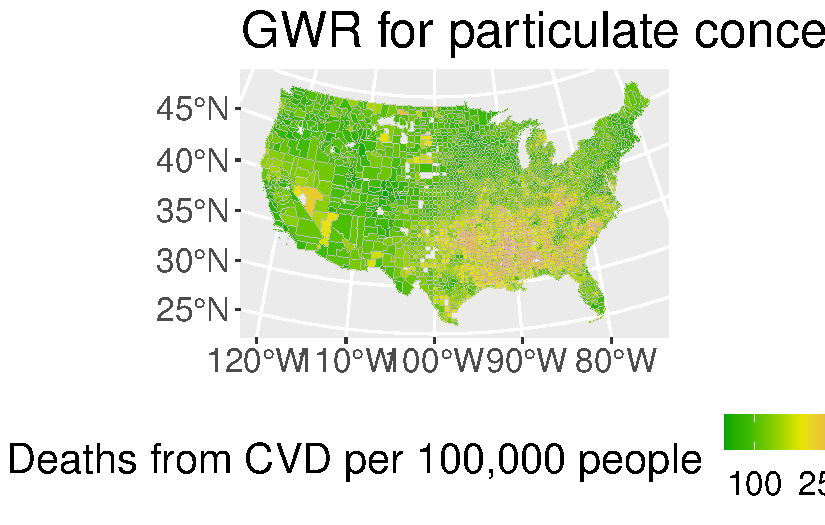
\includegraphics{report_files/figure-pdf/unnamed-chunk-2-1.pdf}

\section{Results}\label{results}

\begin{verbatim}
   ***********************************************************************
   *                       Package   GWmodel                             *
   ***********************************************************************
   Program starts at: 2024-04-22 12:02:53.980286 
   Call:
   gwr.basic(formula = Data_Vl ~ prc_wht + prc_frc + prc_hsp + perc_sn + 
    p2_5_20 + estimat + U__2015, data = mergedf_spatial, bw = opt_bandwidth, 
    kernel = "gaussian", adaptive = FALSE, parallel.method = "omp")

   Dependent (y) variable:  Data_Vl
   Independent variables:  prc_wht prc_frc prc_hsp perc_sn p2_5_20 estimat U__2015
   Number of data points: 3057
   ***********************************************************************
   *                    Results of Global Regression                     *
   ***********************************************************************

   Call:
    lm(formula = formula, data = data)

   Residuals:
     Min       1Q   Median       3Q      Max 
-133.061  -22.813   -5.661   19.637  202.340 

   Coefficients:
                 Estimate Std. Error t value Pr(>|t|)    
   (Intercept)  2.388e+02  1.024e+01  23.313  < 2e-16 ***
   prc_wht     -8.158e+01  9.500e+00  -8.587  < 2e-16 ***
   prc_frc      5.526e+01  9.988e+00   5.532 3.42e-08 ***
   prc_hsp     -9.321e+01  1.023e+01  -9.107  < 2e-16 ***
   perc_sn     -2.090e+02  3.425e+01  -6.101 1.18e-09 ***
   p2_5_20      6.311e+00  4.453e-01  14.170  < 2e-16 ***
   estimat     -2.120e-03  7.150e-05 -29.648  < 2e-16 ***
   U__2015      3.736e+00  4.118e-01   9.072  < 2e-16 ***

   ---Significance stars
   Signif. codes:  0 '***' 0.001 '**' 0.01 '*' 0.05 '.' 0.1 ' ' 1 
   Residual standard error: 35.64 on 3049 degrees of freedom
   Multiple R-squared: 0.6105
   Adjusted R-squared: 0.6096 
   F-statistic: 682.6 on 7 and 3049 DF,  p-value: < 2.2e-16 
   ***Extra Diagnostic information
   Residual sum of squares: 3873809
   Sigma(hat): 35.6093
   AIC:  30534.31
   AICc:  30534.37
   BIC:  27603.76
   ***********************************************************************
   *          Results of Geographically Weighted Regression              *
   ***********************************************************************

   *********************Model calibration information*********************
   Kernel function: gaussian 
   Fixed bandwidth: 128251.7 
   Regression points: the same locations as observations are used.
   Distance metric: Euclidean distance metric is used.

   ****************Summary of GWR coefficient estimates:******************
                    Min.     1st Qu.      Median     3rd Qu.      Max.
   Intercept -1.8237e+02  1.6625e+02  2.7812e+02  4.1353e+02 2293.3931
   prc_wht   -1.7708e+03 -2.3314e+02 -1.1902e+02 -3.3864e+01  309.4663
   prc_frc   -1.9197e+03 -2.0396e+02 -6.1895e+01  5.2242e+01 3229.3222
   prc_hsp   -1.7720e+03 -2.8864e+02 -1.5801e+02 -6.4279e+01  504.0406
   perc_sn   -1.9199e+03 -6.5045e+02 -3.4826e+02 -1.4864e+02 1635.4916
   p2_5_20   -4.8476e+01 -9.9089e-01  3.7131e+00  9.5388e+00   41.5626
   estimat   -8.0369e-03 -2.6333e-03 -1.8226e-03 -1.1243e-03    0.0017
   U__2015   -7.0110e+00  2.6200e+00  5.3167e+00  7.4156e+00   18.3070
   ************************Diagnostic information*************************
   Number of data points: 3057 
   Effective number of parameters (2trace(S) - trace(S'S)): 576.851 
   Effective degrees of freedom (n-2trace(S) + trace(S'S)): 2480.149 
   AICc (GWR book, Fotheringham, et al. 2002, p. 61, eq 2.33): 28146.12 
   AIC (GWR book, Fotheringham, et al. 2002,GWR p. 96, eq. 4.22): 27581.59 
   BIC (GWR book, Fotheringham, et al. 2002,GWR p. 61, eq. 2.34): 27506.99 
   Residual sum of squares: 1290938 
   R-square value:  0.8701873 
   Adjusted R-square value:  0.8399823 

   ***********************************************************************
   Program stops at: 2024-04-22 12:02:54.546821 
\end{verbatim}

\subsection{Table Summary}\label{table-summary}

The analysis compares two statistical models to explore the
relationships between socio-economic, demographic, and environmental
variables and death rates. The first is a global regression model that
does not consider spatial correlation despite revealing that all
predictors are highly statistically significant. Hence, while the model
does suggest that our variables are indeed important, the global model
may overlook local variations that are crucial in understanding the true
nature of the data.

On the other hand, the geographically weighted regression (GWR) model
incorporates spatial variation, which is a critical factor given the
context of the data. We can see how well the GWR model worked by looking
at the R-squared value, which is .870, a significant improvement over
the global model. This R-squared value, along with the use of spatial
statistics, shows the non-uniform relationship between the predictors
and the response variable across different geographical areas. In
summary, by accommodating the spatial component present in the data, the
GWR model provides a more realistic interpretation of how various
factors influence death rates across different regions.

\subsection{Local Significance Plots}\label{local-significance-plots}

In Figure \#1 the plot represents the results of Geographically Weighted
Regression (GWR) analysis of particulate concentrations and their
correlation with cardiovascular disease (CVD) death rates in 2015. The
particulate concentrations include all the covariates mentioned in the
methods section. The regions along the higher latitudes (nearing 45°N)
and towards the eastern section (approaching 80°W) display darker
shades, suggesting higher CVD death rates in these areas, specifically
the midwest and southwest regions.

Figure \#2 represents the local significance and magnitude of the `\%
White' demographic parameter on cardiovascular disease outcomes. From
the plot, the prominent dark purple areas in the central part of the
country, extending towards the southeastern regions, indicate a
significant negative correlation between the percentage of the white
population and CVD outcomes in these areas. Same with the Northwest
region, however, there are few areas, particularly in the southwest near
New Mexico and Arizona, where there are positively correlated to CVD
death rate, with the white regions of counties suggesting no
significance.

Figure \#3 represents the local significance and magnitude of the `\%
African' demographic parameter on cardiovascular disease outcomes. From
the plot, areas located approximately in the northern central region
indicate a significant positive correlation to CVD rate, and areas,
notably in the central to southeastern areas of the map, suggest a
significant negative correlation, with the white regions of counties
suggesting no significance.

Figure \#4 represents the local significance and magnitude of the `\%
Hispanic' demographic parameter on cardiovascular disease outcomes. From
the plot, areas across the central and southeastern regions are shaded
in purple, suggesting a significant negative correlation between the
percentage of the Hispanic population and CVD outcomes. There are
isolated red patches in the north-central region, indicating areas where
an increased percentage of the Hispanic population correlates with
higher CVD outcomes. Lastly, as per the last figure, the white regions
are specified as having no significance.

Figure \#5 represents the local significance and magnitude of the `\%
Asian' demographic parameter on cardiovascular disease outcomes. From
the plot, a substantial portion of the map, particularly across the
central to eastern regions, is colored in various shades of purple. This
suggests that in these areas, an increased percentage of the Asian
population correlates with lower CVD outcomes. However, there are some
parts of the West where higher percentages of the Asian population are
associated with an increase in CVD outcomes.

Figure \#6 represents the local significance and magnitude of the
``\%p2.5 air quality'' parameter on cardiovascular disease outcomes.
From the plot, in the southern and northeastern regions, there increased
levels of PM2.5 colored as red in the plot, meaning they are associated
with higher rates of CVD. There are some regions in the West where it
was negatively correlated with CVD. As usual, the white areas signify no
significance.

Figure \#7 represents the local significance and magnitude of the
``median income'' parameter on cardiovascular disease outcomes. From the
plot, most of the region suggests that there is significant negative
correlation between the median income parameter and CVD outcomes.
However, some parts of Texas indicate a positive correlation to CVD
outcomes. As usual, the white areas signify no significance.

Figure \#8 represents the local significance and magnitude of the
``Unemployment'' parameter on cardiovascular disease outcomes. From the
plot, in most of the central region, there is a positive correlation to
CVD rates, and in the southwest region, you can see a negative
correlation to CVD rates. As usual, the white areas signify no
significance.

\begin{figure}

\begin{minipage}{0.50\linewidth}
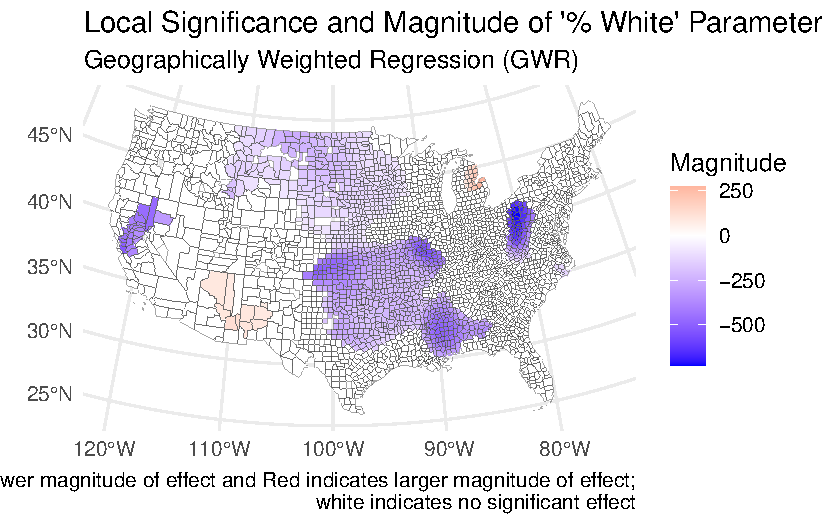
\includegraphics{report_files/figure-pdf/unnamed-chunk-4-1.pdf}\end{minipage}%
%
\begin{minipage}{0.50\linewidth}
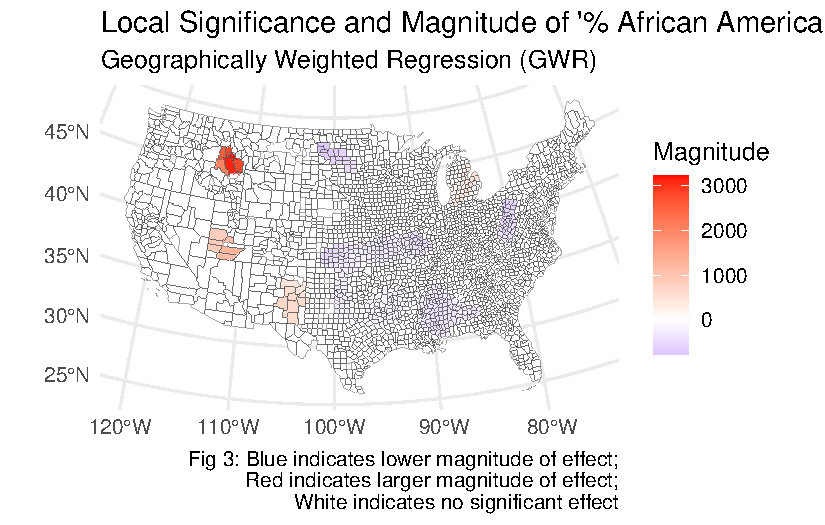
\includegraphics{report_files/figure-pdf/unnamed-chunk-4-2.pdf}\end{minipage}%
\newline
\begin{minipage}{0.50\linewidth}
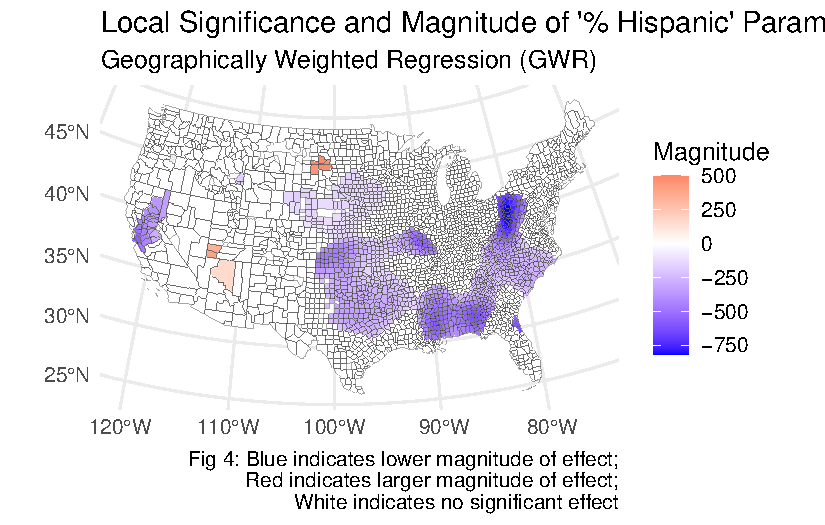
\includegraphics{report_files/figure-pdf/unnamed-chunk-4-3.pdf}\end{minipage}%
%
\begin{minipage}{0.50\linewidth}
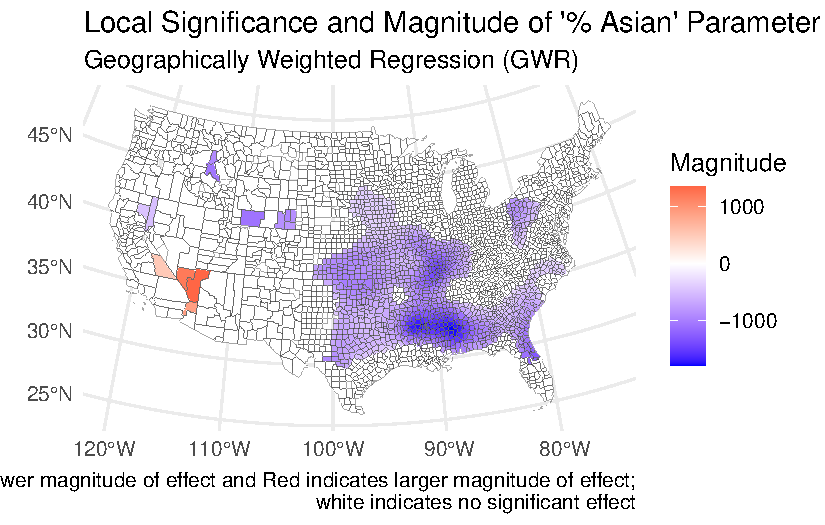
\includegraphics{report_files/figure-pdf/unnamed-chunk-4-4.pdf}\end{minipage}%

\end{figure}%

\begin{itemize}
\tightlist
\item
  Demographic Impact: The percentage of white and Hispanic populations
  shows significant regional variations in association with death rates.
  Higher proportions of white populations correlate with lower death
  rates in central areas, whereas higher percentages of Hispanic
  populations are linked to lower death rates in the West and Southwest.
  Conversely, higher percentages of African American populations are
  associated with higher death rates in certain Midwestern and
  Southeastern regions.
\end{itemize}

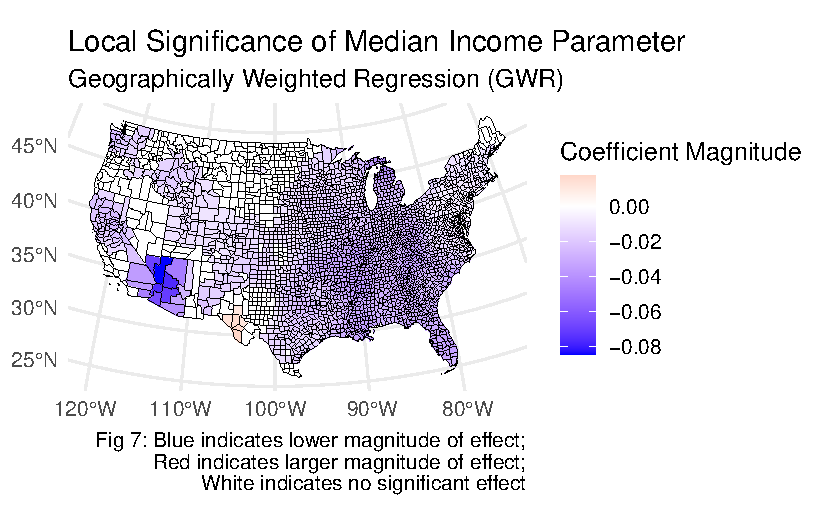
\includegraphics{report_files/figure-pdf/unnamed-chunk-5-1.pdf}

\begin{itemize}
\tightlist
\item
  Environmental Influence: Air quality, indicated by PM2.5 levels,
  demonstrates a significant positive relationship with death rates,
  particularly east of the Rockies, highlighting environmental health as
  a major concern.
\end{itemize}

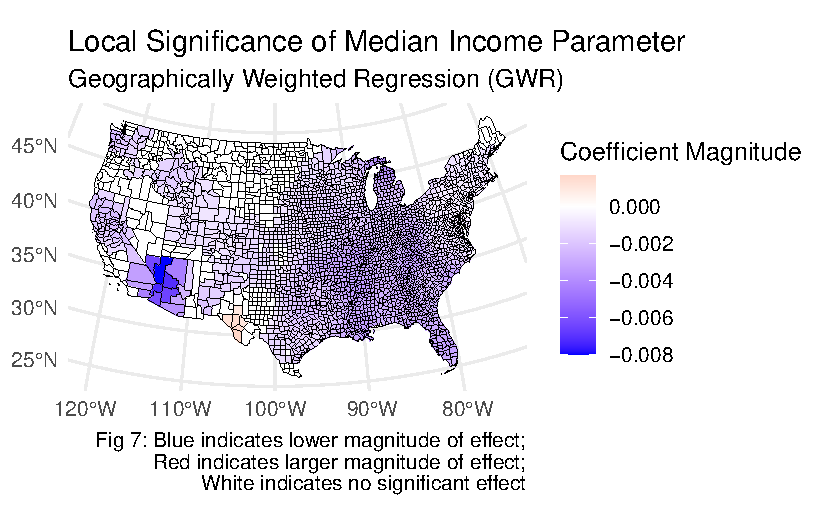
\includegraphics{report_files/figure-pdf/unnamed-chunk-6-1.pdf}

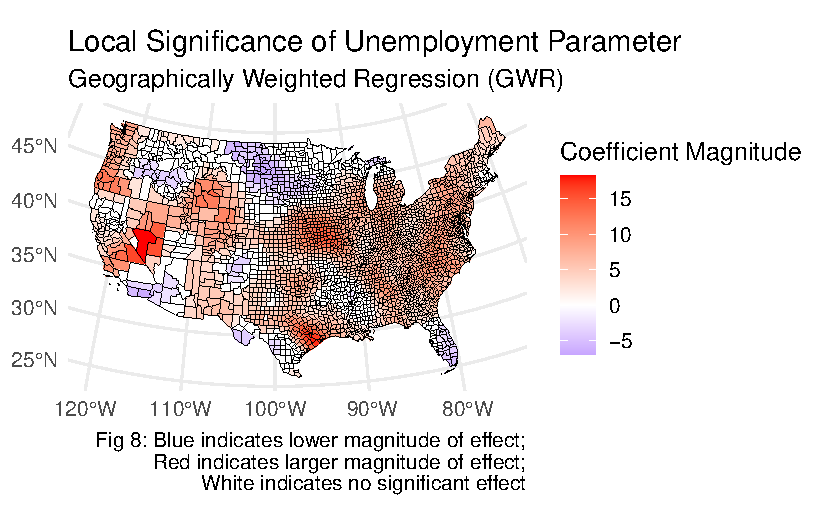
\includegraphics{report_files/figure-pdf/unnamed-chunk-6-2.pdf}

\begin{itemize}
\tightlist
\item
  Socio-economic Correlation: Median income levels across many regions
  show a consistent negative association with death rates, suggesting
  that higher income areas generally experience fewer deaths.
\end{itemize}

\section{Discussion}\label{discussion}

The purpose of this study was to fill a gap in prior studies where the
impacts of CVD were primarily studied within the Stroke Belt, rather
than the country at large.

Our goal was to put our findings towards answering the following
question: what are the socioeconomic and environmental factors affecting
CVD rates in the United States?

These maps reveal that the relationships between race, socio-economic
factors, environmental quality, and death rates are complex and highly
localized. The significance and strength of these relationships vary
considerably across different parts of the United States. In contrast,
some of the socio-economic factors such as median income show
widespread, consistent significance, implying that the significance of
the relationship with CVD outcomes is nearly constant across various
locations. This differs from the heterogeneous local significance that
we observed in the majority of our other variables.

Another factor to consider from the plots is the percentage of each race
that inhabits each county. We can observe that for African Americans,
Hispanics, and Asians that the impacts are significant in localized
areas of the country, which may reflect underlying health disparities in
access to medical care.

\begin{itemize}
\tightlist
\item
  One limitation of race percentages is the misreporting of medical
  records affecting minorities (Tabb et al.) However, this oversight
  lends further credence to the fact that intervention is needed in
  order to combat racial health disparities. We can look at the Variance
  Inflation Factor (VIF) to show that the multicollinearity does not
  impact our results:
\end{itemize}

Concentration of PM2.5 and the consequential reduction in air quality
has a significant impact localized in the central and southeastern
regions of the United States, suggesting environmental health concerns
that might require region-specific intervention.~

We have shown that by using a GWR model to analyze the relationship
between CVM and socioeconomic covariates, the factors that have the most
significant impact on death rates vary by area of the country. This
highlights the need to identify efficient methods of intervention in
order to curb one of the deadliest groups of diseases on the planet
(Marlow 1994).

\newpage{}

\section*{References}\label{references}
\addcontentsline{toc}{section}{References}

\phantomsection\label{refs}
\begin{CSLReferences}{1}{0}
\bibitem[\citeproctext]{ref-gebreabExploringRacialDisparities2012}
Gebreab, Samson Y., and Ana V. Diez Roux. 2012. {``Exploring Racial
Disparities in {CHD} Mortality Between Blacks and Whites Across the
{United} {States}: {A} Geographically Weighted Regression Approach.''}
\emph{Health \& Place} 18 (5): 1006--14.
\url{https://doi.org/10.1016/j.healthplace.2012.06.006}.

\bibitem[\citeproctext]{ref-Marlow1994}
Marlow, Hilary F. 1994. {``The Pharmaceutical Industry Viewpoint.''}
\emph{Cardiology} 85 (1): 102--12.
\url{https://doi.org/10.1159/000176769}.

\bibitem[\citeproctext]{ref-singhSpatiotemporalDemographicTrends2019}
Singh, Gitanjali M., Ninon Becquart, Melissa Cruz, Andrea Acevedo,
Dariush Mozaffarian, and Elena N. Naumova. 2019. {``Spatiotemporal and
{Demographic} {Trends} and {Disparities} in {Cardiovascular} {Disease}
{Among} {Older} {Adults} in the {United} {States} {Based} on 181
{Million} {Hospitalization} {Records}.''} \emph{Journal of the American
Heart Association} 8 (21): e012727.
\url{https://doi.org/10.1161/JAHA.119.012727}.

\bibitem[\citeproctext]{ref-terryTrendsCardiovascularDisease2023}
Terry, Katrina, Mohamed Makhlouf, Salah E. Altarabsheh, Vaishali Deo,
Fanny Petermann-Rocha, Yakov Elgudin, Khurram Nasir, Sanjay Rajagopalan,
Sadeer Al-Kindi, and Salil Deo. 2023. {``Trends in {Cardiovascular}
{Disease} {Mortality} by {County}-{Level} {Social} {Vulnerability}
{Index} in the {United} {States}.''} \emph{Journal of the American Heart
Association} 12 (20): e030290.
\url{https://doi.org/10.1161/JAHA.123.030290}.

\bibitem[\citeproctext]{ref-zelkoGeographicallyWeightedModeling2023}
Zelko, Andrea, Pedro R. V. O. Salerno, Sadeer Al-Kindi, Fredrick Ho,
Fanny Petermann Rocha, Khurram Nasir, Sanjay Rajagopalan, Salil Deo, and
Naveed Sattar. 2023. {``Geographically {Weighted} {Modeling} to
{Explore} {Social} and {Environmental} {Factors} {Affecting}
{County}-{Level} {Cardiovascular} {Mortality} in {People} {With}
{Diabetes} in the {United} {States}: {A} {Cross}-{Sectional}
{Analysis}.''} \emph{The American Journal of Cardiology} 209 (December):
193--98. \url{https://doi.org/10.1016/j.amjcard.2023.09.084}.

\end{CSLReferences}



\end{document}
